Dovetailing into the non-monotonicity of the ACT's Intouchpoints is a similar behavior by $X_{88}$, the Isogonal Conjugate of $X_{44}$, known to lie on the EB and to be to be collinear with $X_1$ and $X_{100}$, \cite{etc}. The latter is verified by the vanishing determinant of the 3x3 matrix whose rows are the trilinears of $X_1,X_{100},X_{88}$  \cite[under ``Collinear'', eqn 9]{mw}:

\[
\det\left[
\begin {array}{ccc}
1&1&1\\
 \frac{1}{s_2-s_3} & \frac{1}{s_3-s_1} & \frac{1}{s_1-s_2} \\ 
\frac{1}{s_2+s_3-2\,s_1}& \frac{1}{s_1+s_3-2\,s_2} & \frac{1}{s_1+s_2-2\,s_3}
\end{array}
\right]{\equiv}\,0
\]

\smallskip

Furthermore $X_{100}$ is a very special point: it lies on the EB and on the Circumcircle simultaneously \cite{etc}. Let $\alpha_{88}=(\sqrt{6+2\sqrt{2}}\,)/2\simeq{1.485}$.

\begin{proposition}
At $a/b=\alpha_{88}$, the y velocity of $X_{88}$ vanishes when the 3-periodic is a sideways isosceles.
\end{proposition}

\begin{proof}
Parametrize $P_1(t)$ in the usual way. At $t=0$, $P_1=(a,0)$ it can be easily checked that $X_{88}=(-a,0)$. Solve $y_{88}'(t)|_{t=0}=0$ for $a/b$. After some algebraic manipulation, this equivalent to solving $4x^4-12x^2+7=0$, whose positive roots are $(\sqrt{6\pm 2\sqrt{2}}\,)/2$. $\alpha_{88} $ is the largest of the two.
\end{proof}

As shown in Table~\ref{tab:x88}, there are three types of $X_{88}$ motion with respect to $P_1(t)$: monotonic, with stops at the EB vertices, and non-monotonic.


\begin{table}
\begin{center}
\small
\begin{tabular}{|c|l|l|}
\hline
$a/b$ vs. $\alpha_{88}$ & motion & comment \\
\hline
$<$ & CW & monotonic\\
$=$ & CW & stops at EB vertices \\
$>$ & CW+CCW & non-monotonic \\
\hline
\end{tabular}
\caption{Conditions for the type of motion of $X_{88}$ with respect to $P_1(t)$. \textbf{Video}: \cite[PL\#11]{reznik2020-playlist-intriguing}}
\label{tab:x88}
\end{center}
\end{table}


An equivalent statement is that the line family $X_1X_{100}$ is instantaneously tangent to its {\em envelope} \cite{mw} at $X_{88}$. Figure~\ref{fig:x88-envelope} shows that said envelope lies (i) entirely inside, (ii) touches at vertices of, or (iii) is partially outside, the EB, when $a/b$ is less than, equal, or greater than $\alpha_{88}$, respectively. Each such case implies the motion of $X_{88}$ is (i) monotonically opposite to $P_1(t)$, (ii) opposite but with stops at the EB vertices, or (iii) is non-monotonic.

The reader is challenged to find an expression for parameter $t$ in $P_1(t)$ where the motion of $X_{88}$ changes direction. The following additional facts are also true for $X_{88}$:

\begin{proposition}\label{prop:x88}
$X_{88}$ coincides with a 3-periodic vertex if and only if $s_2 = (s_1+s_3)/2$. In this case, $X_1$ is the midpoint between $X_{100}$ and $X_{88}$ \cite{helman2020-private-x88}, Figure~\ref{fig:x88tri} (bottom left).
\end{proposition}

\begin{proof}
The first trilinear coordinate of $X_{88}$ is $1/(s_2 + s_3 - 2 s_1)$ \cite{etc}, and of a vertex is $0$. Equating the two yields $s_2 = (s_1+s_3)/2$.
Consider a triangle of reference $P_1=(-1,0)$, $P_2=(u,v)$, $P_3=(1,0)$. Its circumcircle is given by  $v(x^2+y^2)+(1-u^2-v^2)y-v=0.$ Under the hypothesis $s_2=(s_1+s_3)/2$ it follows that $v=\sqrt{12-3u^2}/2$, $s_1=2-u/2$, $s_2=2$ and $s_3=2+u/2$.  Therefore the incenter is   $ I= (s_1P_1+s_2P_2+s_3P_3)/(s_1+s_2+s_3)=(u/2, \sqrt{12-3u^2}/6)$. The intersection of the straight line passing through $P_2$ and $I$ with the circumcircle of the triangle o reference is the point $D=(0,\sqrt{12-3u^2}/6).$
Therefore, $I$ is the midpoint of $B$ and $D=X_{100}$. Moreover, $\mid P_1-D\mid=\mid P_2-D\mid=\mid I-D\mid= \sqrt{48-3u^2}/6$.
\end{proof}
%
\begin{figure}
    \centering
    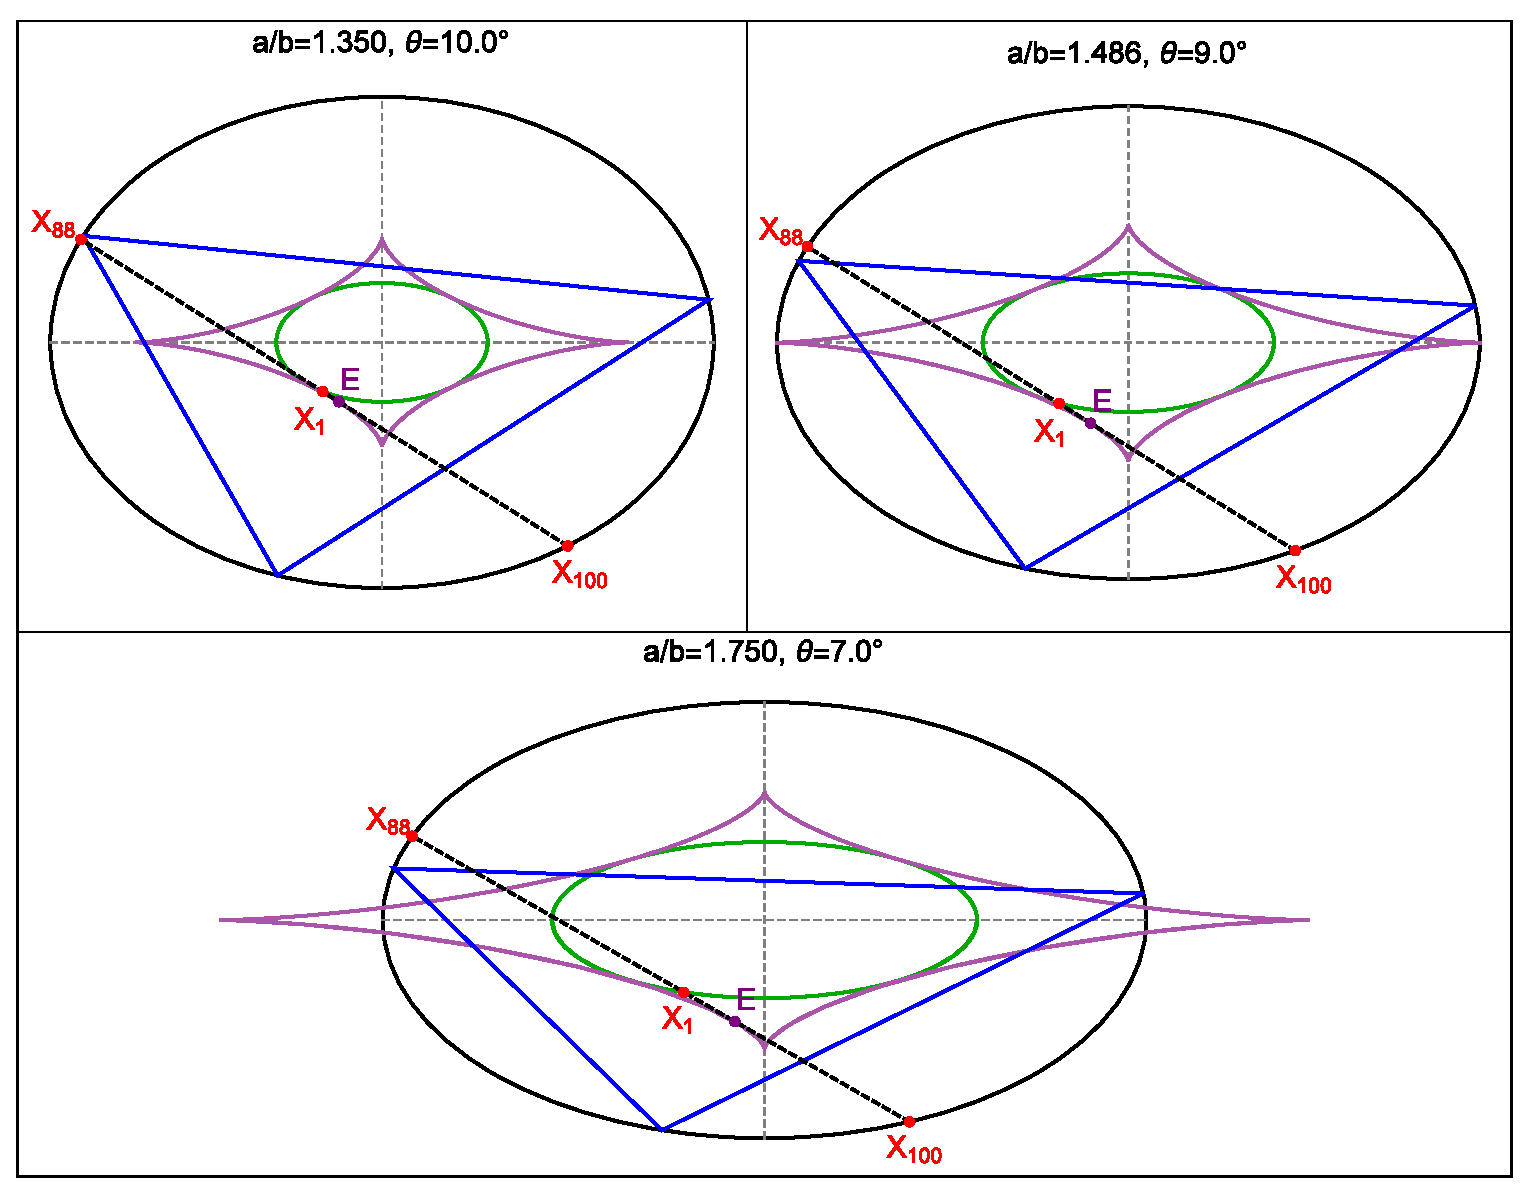
\includegraphics[width=\textwidth]{pics/1120_x88_trio.eps}
    \caption{Collinear points $X_1,X_{100},X_{88}$ shown for billiards with $a/b$ less than (top-left), equal (top-right), or greater (bottom) than $\alpha_{88}{\simeq}1.486$, respectively. In each such case, the motion of $X_{88}$ relative to the 3-periodic vertices will be monotonic, with stops at the vertices, or non-monotonic, respectively. Equivalently, the motion of $X_{88}$ is opposite to $P_1$, stationary, or in the direction of $P_1$ if the instantaneous center of rotation $E$ of line $X_1X_{100}$ lies inside, on, or outside the EB. The locus of $E$ (the envelope of $X_1X_{100}$) is shown purple. Notice it only ``pierces'' the EB when $a/b>\alpha_{88}$ (bottom), i.e., only in this case can the motion of $X_{88}$ be non-monotonic. \textbf{Video}: \cite[PL\#12]{reznik2020-playlist-intriguing}}
    \label{fig:x88-envelope}
\end{figure}
%
It is well-known that the only right-triangle with one side equal to the average of the other two is $3:4:5$. Let $\alpha_{88}^\perp=(7+\sqrt{5})\sqrt{11}/22\simeq{1.3924}.$  Referring to Figure~\ref{fig:x88tri} (right):

\begin{proposition}
The only EB which can contain a 3:4:5 3-periodic has an aspect ratio $a/b=\alpha_{88}^\perp$.
\end{proposition}

\begin{proof}
With $a/b>\alpha_4=\sqrt{2\,\sqrt{2}-1}\simeq{1.352}$ the 3-periodic family contains obtuse triangles amongst which there always are 4 right triangles (identical up to rotation and reflection). Consider the elementary triangle $P_1=(0,0)$, $P_2=(s_1,0)$, and $P_3=(s_1,s_2)$ choosing $s_1,s_2$ integers such that $s_3=s_3=\sqrt{s_1^2+s_2^2}$ is an integer. The Circumbilliard \cite{garcia2020-new-properties} is given by:
%
\[
E_9(x,y)= s_2 x^2+ \left( s_3-s_1-s_2 \right) xy+s_1{y}^{2}-s_1s_2x-s_1 \left( s_1-s_3 \right) y=0.\]
%
Squaring the ratio of the Eigenvalues of $E_9$'s Hessian yields the following expression for $a/b$:
%
\begin{equation}
    [a/b](s_1,s_2,s_3)= \frac {s_1+s_2+\sqrt {s_3\left(3\,s_3-2\,s_1-2\,s_2\right) }}{\sqrt { \left( 
s_1+s_2+3\,s_3 \right)  \left( s_1+s_2-s_3 \right) }}
\end{equation}
\end{proof}

%The sides $s_1,s_2,s_3$ of a right triangle are related as %sides $s_1,s_2,s_3$ for which $s_1,s_2$ are co-prime, and %$s_3^2=s_1^2+s_2^2$.


\noindent Table~\ref{tab:pythagorean} shows $a/b$ for the first 5 Pythagorean triples ordered by hypotenuse\footnote{The $a/b$ which produces $3:4:5$ was first computed in connection with $X_{88}$ \cite{helman2020-private-x88}.}.
%
{\small  
\begin{table}
$$
\begin{array}{r|c|l|l}
(s_1,s_2,s_3) & a/b & {\simeq}a/b \\
\hline
3, 4, 5 & {(7+\sqrt{5})\sqrt{11}}/{22} &  1.392  \\
5, 12, 13 & {\sqrt{14} (\sqrt{65}+17)}/{56} & 1.674  \\
8, 15, 17 & {\sqrt{111} (\sqrt{85}+23)}/{222} & 1.529 \\
7, 24, 25  & {\sqrt{159} (5\,\sqrt{13}+31)}/{318} & 1.944 \\
20, 21, 29 & \sqrt{6} (\sqrt{145}+41)/{96} & 1.353 &   \\
\end{array}
$$
%\[a/b_{\perp}(m,n,p)=\sqrt {{\frac {m+n+\sqrt {p %( -2\,m-2\,n+3\,p \right) }}{m+n-
%\sqrt {p ( -2\,m-2\,n+3\,p \right) }}}}\]
\caption{First 5 Pythagorean triples ordered by hypotenuse. $a/b$ is the aspect ratio.
of the EB which produces 4 triangles homothetic to the triple.}
\label{tab:pythagorean}
\end{table}
}

\begin{figure}
    \centering
    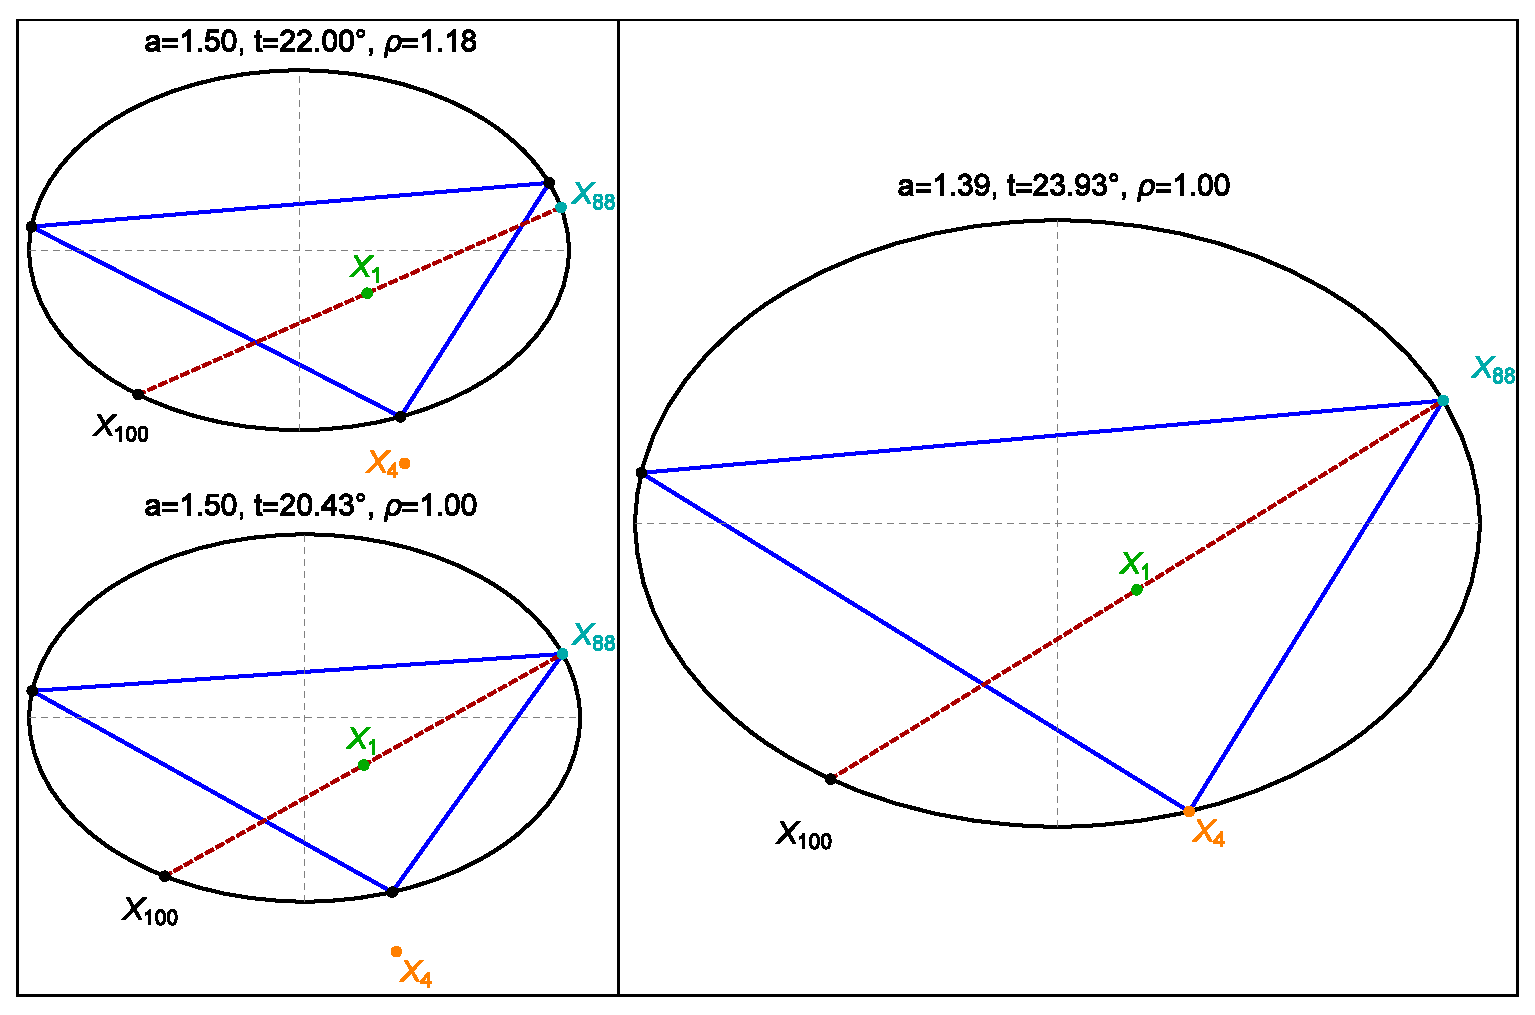
\includegraphics[width=\textwidth]{pics/1130_x88_both.eps}
    \caption{$X_{88}$ is always on the EB and collinear with $X_1$ and $X_{100}$ \cite{etc}. Let $\rho$ (shown above each picture) be the ratio $|X_1-X_{100}|/|X_1-X_{88}|$. \textbf{Top Left}: The particular 3-periodic shown is obtuse ($X_4$ is exterior), and $\rho>1$, i.e., $X_1$ is closer to $X_{88}$. \textbf{Bottom Left}: When $X_{88}$ coincides with a vertex, if sidelengths are ordered as $s_1{\leq}s_2{\leq}s_3$, then $s_2=(s_1+s_3)/2$, and $X_1$ becomes the midpoint of $X_{88}X_{100}$, i.e., $\rho=1$. \textbf{Right}: If $a/b=\alpha_{88}^\perp\,{\simeq}\,1.39$, when $X_{88}$ is on a vertex, the 3-periodic is a $3:4:5$ triangle ($X_4$ lies on an alternate vertex). \textbf{Video}: \cite[PL\#11]{reznik2020-playlist-intriguing}}
    \label{fig:x88tri}
\end{figure}

\begin{figure}
    \centering
    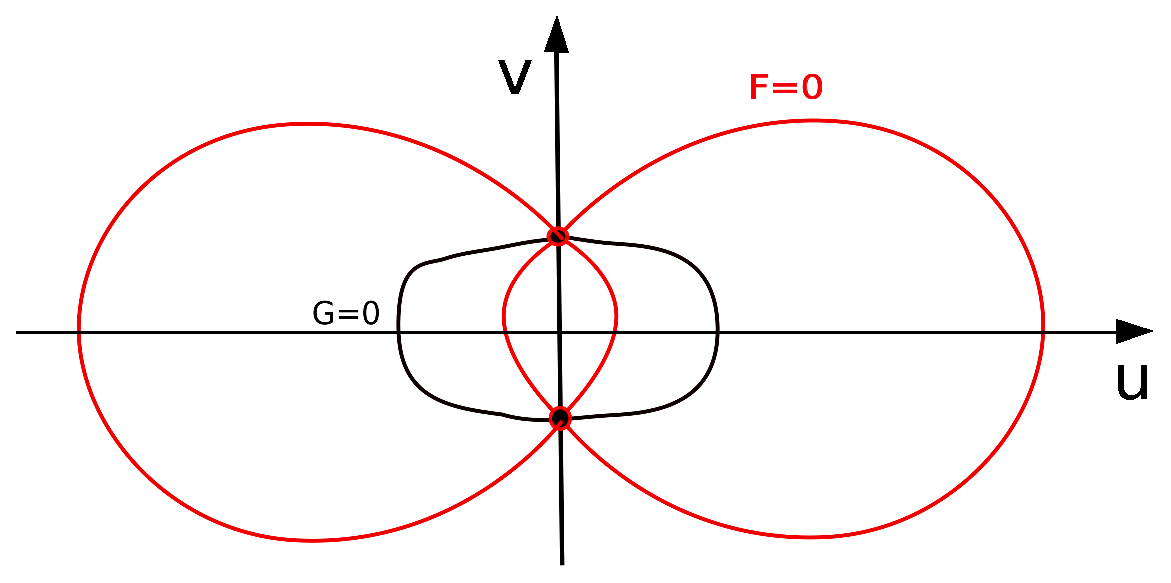
\includegraphics[width=.66\textwidth]{pics/1140_x88x162_level_curves.eps}
    \caption{Level curves $F=0$ (red) and $G=0$ (black). }
    \label{fig:x88x162}
\end{figure}